\section{Knowledge Management - I Lecture}

\subsection{Introduction to Knowledge
    Management}\label{introduction-to-knowledge-management}

Good morning everyone! In this class, our main focus will be on
knowledge management.

\begin{figure}[!h]
    \centering
    \includegraphics[page=2, trim = 1.5cm 7cm 3cm 4.5cm, clip, width=\textwidth]{images/05 - KM.pdf}
\end{figure}

So, what exactly is knowledge management? It refers to the effective
management of knowledge within organizations.

\subsection{Defining Knowledge}\label{defining-knowledge}

\begin{figure}[!h]
    \centering
    \includegraphics[page=3, trim = 1.5cm 3cm 3cm 3.5cm, clip, width=\textwidth]{images/05 - KM.pdf}
\end{figure}

The concept of knowledge is multifaceted and has been extensively
explored in literature. It can be defined in various ways, depending on
the context. Knowledge can be seen as a state of mind, an object, a
process, a capability, or even as the transformation of information into
something practical that can solve real-world problems. The definitions
of knowledge span across different disciplines, from philosophy to
engineering and coding.

\subsection{Knowledge Management in Service
    Companies}\label{knowledge-management-in-service-companies}

In the context of service companies, knowledge management plays a
crucial role in improving service quality and personalization. It
involves the collection, structuring, and transformation of information
gathered during service operations into valuable knowledge for future
activities. By effectively managing this process, service companies can
maintain a strong relationship with their market and easily adapt to
changing market requirements.

For instance, one question that often arises in knowledge management is
how to embed company knowledge into software. This topic was initially
introduced in the Business Information Systems (BIS I) course,
specifically when discussing service companies. In this context,
knowledge management was defined as the process through which service
companies gather information during their service operations. This
includes interactions with customers and the completion of back-office
operations to deliver services. The collected information is then
structured and transformed into knowledge that can be utilized to
enhance the quality and personalization of future service activities.

It is important to note that when knowledge management is effectively
implemented, service companies can maintain a close relationship with
their market. This enables them to adapt their services to meet new
market requirements as they arise.

\subsection{Evolution and Definitions in IT
    Context}\label{evolution-and-definitions-in-it-context}

\begin{figure}[!h]
    \centering
    \includegraphics[page=4, trim = 1.5cm 4cm 1.5cm 4.5cm, clip, width=\textwidth]{images/05 - KM.pdf}
\end{figure}

In the context of knowledge management, knowledge is seen as a practical
tool for companies. It allows them to give meaning to data and address
organizational issues, especially in terms of continuous learning,
managing new requirements, and adapting to market changes. The concept
of knowledge management in service companies was initially defined in
the mid-90s and has been periodically revisited as new technologies
emerge. While there have been various definitions, when considering the
application of information technology, there is a general consensus on a
few key factors. Firstly, knowledge is closely connected to information
and represents a transformation of that information, which itself is a
transformation of data.

\subsection{Knowledge Transformation and Practical
    Application}\label{knowledge-transformation-and-practical-application}

In the process of knowledge transformation, data is first collected and
structured to obtain information. However, simply possessing information
is not enough to guarantee knowledge within a company. Knowledge is
derived from information, but it also requires the ability to transform
that information into something useful. In the context of service
companies, knowledge is closely tied to change and finding creative
solutions to new problems. As the market evolves, companies must adapt
and apply their knowledge in a creative way to solve specific problems
in unique situations. It's important to note that this knowledge is not
purely theoretical, but rather directly tied to action. The purpose of
creating knowledge is to support actions, make informed choices, and
drive innovation.

\subsection{Taxonomy of Knowledge}\label{taxonomy-of-knowledge}

\begin{figure}[!h]
    \centering
    \includegraphics[page=5, trim = 1.5cm 1cm 1.5cm 3cm, clip, width=\textwidth]{images/05 - KM.pdf}
\end{figure}

\subsubsection{Internal vs.~External
    Knowledge}\label{internal-vs.-external-knowledge}

In addition to the principles we discussed earlier, it is important to
understand the taxonomy of knowledge. This taxonomy helps classify
different types of knowledge and provides a framework for leveraging
knowledge to drive innovation. One key distinction is between internal
and external knowledge.

Internal knowledge refers to the knowledge that exists within the
boundaries of a company. It is the knowledge that the company possesses
and has developed over time. On the other hand, external knowledge is
knowledge that comes from outside the company's boundaries. This can be
obtained through various means, such as hiring consultants or purchasing
information from external sources.

For example, companies can hire consultants who bring their expertise
and knowledge to help solve specific problems or provide guidance. They
can also purchase information from information providers to gain
insights and access to data that can be used for various purposes,
including data monetization.

Understanding the difference between internal and external knowledge is
crucial for companies to effectively utilize knowledge and drive
innovation. By leveraging both internal and external knowledge,
companies can tap into a wider range of expertise and resources to stay
competitive and foster creativity.

\subsubsection{Personal vs.~Organizational
    Knowledge}\label{personal-vs.-organizational-knowledge}

Another important distinction in the taxonomy of knowledge is between
personal and organizational knowledge. Personal knowledge refers to the
knowledge that individuals possess in their minds. When working for an
organization, the knowledge that an individual acquires and applies is
their personal knowledge. On the other hand, organizations also possess
collective knowledge. Organizations are created with the purpose of
achieving specific objectives that no single individual can accomplish
alone. This collective knowledge encompasses not only the sum of
individual knowledge within the organization but also includes
methodologies, strategies, best practices, and processes that the
organization employs to achieve its objectives. It is the way in which
individual knowledge is combined and utilized to solve problems and
reach organizational goals.

The existence of collective knowledge in organizations is significant.
It allows organizations to create value that goes beyond the
capabilities of individual employees. By leveraging this collective
knowledge, organizations can achieve outcomes that would be difficult to
attain solely by hiring individuals. Additionally, the presence of
collective knowledge ensures that if an individual leaves the
organization, their knowledge can be replaced and the organization can
still continue to pursue its objectives.

\subsubsection{Tacit vs.~Explicit
    Knowledge}\label{tacit-vs.-explicit-knowledge}

In the taxonomy of knowledge, there is a clear distinction between tacit
and explicit knowledge. Tacit knowledge refers to knowledge that is
difficult to articulate or codify. It resides within the minds of
individuals and is challenging to transfer to others. On the other hand,
explicit knowledge can be easily documented and shared. For instance,
one can write a book on a specific subject, but the readers cannot
acquire the same level of expertise as the author.

This differentiation highlights the limitations of formal education, as
there are certain aspects of knowledge that cannot be fully captured in
books or taught in a classroom. However, companies make significant
efforts to convert tacit knowledge into explicit knowledge whenever
possible. This is done to ensure that if an individual leaves the
organization, their knowledge can be easily replaced and transferred to
new employees. The goal is to expedite the process of acquiring
expertise for new hires and minimize any potential disruptions.

\subsection{Knowledge as a Resource}\label{knowledge-as-a-resource}

\begin{figure}[!h]
    \centering
    \includegraphics[page=6, trim = 1.5cm 2.8cm 1.5cm 4cm, clip, width=\textwidth]{images/05 - KM.pdf}
\end{figure}

Knowledge is a valuable resource for companies, as it can provide a
sustained competitive advantage. The resource-based view of the firm
(RBV) considers organizations as a collection of resources, with
knowledge being one of them. The RBV theory aims to categorize resources
and determine which ones are crucial for a company's success and
competitive advantage.

When evaluating knowledge as a resource, it is important to consider
whether it can be easily obtained from the market. If a certain type of
knowledge is readily available for purchase, it cannot be a reliable
source of sustained competitive advantage. While it may still be
important, it is not a key factor in differentiating the company from
its competitors.

\begin{figure}[!h]
    \centering
    \includegraphics[page=7, trim = 1.5cm 2cm 1.5cm 3cm, clip, width=\textwidth]{images/05 - KM.pdf}
\end{figure}

The RBV framework is commonly used to rank and assess the resources of a
company. It can even be used to evaluate the overall value of a company
in the markek. By examining the intrinsic value, rarity, imitability,
and substitutability of the company's resources, including knowledge,
one can determine their impact on sustained competitive advantage. A
company with rare, difficult-to-replicate, and irreplaceable resources
holds greater value.

A Sustainable Competitive Advantage (SCA) is a competitive edge that a firm can maintain over time by exploiting its unique resources and capabilities. It is a result of a firm's ability to use its resources and capabilities in a way that is not easily imitated or substituted by competitors. The RBV theory emphasizes that not all resources are of equal importance, nor do they possess the potential to become a source of SCA. The sustainability of any competitive advantage depends on the extent to which resources can be imitated or substituted.

In summary, knowledge is a valuable resource for companies, but its true
worth lies in its rarity, imitability, and inability to be easily
replaced by competitors. This can include unique
personal skills or specialized organizational knowledge that is
difficult to imitate or replace. Access to knowledge can even serve as a
barrier to entry for competitors in a particular market segment. The RBV framework provides a useful tool for evaluating the importance of knowledge and other resources in achieving
sustained competitive advantage (SCA).

\subsection{Managing Knowledge}\label{managing-knowledge}

\subsubsection{Complexity and Integrated
    View}\label{complexity-and-integrated-view}

\begin{figure}[!h]
    \centering
    \includegraphics[page=8, trim = 1.5cm 5cm 1.5cm 4.5cm, clip, width=\textwidth]{images/05 - KM.pdf}
\end{figure}

Managing knowledge is a complex task that requires an integrated view of
the organization. It involves using information to improve the company's
ability to achieve its objectives. This requires a cross-divisional and
enterprise-wide approach, as discussed in BIS1. Creating virtuous cycles
within the company, where information is used to generate new knowledge
and drive growth, is a challenging but essential aspect of knowledge
management.

\subsubsection{Technocratic, Economic, and Behavioral
    Perspectives}\label{technocratic-economic-and-behavioral-perspectives}


\begin{figure}[!h]
    \centering
    \includegraphics[page=9, trim = 1.5cm 4.5cm 1.5cm 3.5cm, clip, width=\textwidth]{images/05 - KM.pdf}
\end{figure}

Even as companies experience growth and innovation in their early
stages, they often struggle to maintain this capability as they expand.
This is why large corporations not only innovate internally but also
acquire startups. It is challenging for them to maintain a constant flow
of fresh ideas and motivate and reward innovators in a sustainable way.
However, companies always strive to create social incentives for
knowledge sharing, even if it is difficult. They want to ensure that
individuals do not hoard knowledge but instead share it as much as
possible, and they provide rewards for doing so. Knowledge management
systems play a crucial role in facilitating this process. The main
application of information technology in this context is to create an
environment that encourages knowledge sharing and growth.

Managing knowledge can be approached from different perspectives:
technocratic, economic, and behavioral. These perspectives are not
mutually exclusive and are often used in combination. All three
perspectives must be applied to effectively perform knowledge management
in companies. The technocratic view focuses on how information
technology can support knowledge processes. The economic view emphasizes
evaluating and monetizing knowledge, as well as assigning and monitoring
its value within the company. The behavioral view addresses how to
manage and create social incentives to promote knowledge sharing and the
continuous growth of organizational knowledge.

\subsubsection{Technocratic Strategy}\label{technocratic-strategy}

\begin{figure}[!h]
    \centering
    \includegraphics[page=10, trim = 1.5cm 6.5cm 1.5cm 3.5cm, clip, width=\textwidth]{images/05 - KM.pdf}
\end{figure}

In the technocratic strategy, the focus is on technology and addressing
the fundamental problem of capturing and sharing information to create
knowledge. One key question is how to ensure that the necessary
information is available to everyone. Formalizing techniques for risk
assessment in insurance companies is an example of how knowledge can be
captured and made accessible to others. Another example is the use of
information technology tools like Slack, which facilitate cooperation,
knowledge sharing, and keeping everyone updated on different issues.

\subsubsection{Economic Strategy}\label{economic-strategy}

\begin{figure}[!h]
    \centering
    \includegraphics[page=11, trim = 1.5cm 2.8cm 1.5cm 4.5cm, clip, width=\textwidth]{images/05 - KM.pdf}
\end{figure}

In the context of economic strategy, the focus is on managing knowledge
as a valuable asset. This involves utilizing various mechanisms to
protect knowledge within organizations, such as patents, copyright, NDAs
(non-disclosure agreements), intellectual property management, and trade
secrets. These tools ensure that knowledge remains safeguarded and
secure.

\subsubsection{Behavioral Strategy}\label{behavioral-strategy}

\begin{figure}[!h]
    \centering
    \includegraphics[page=12, trim = 1.4cm 5cm 1.5cm 3.7cm, clip, width=\textwidth]{images/05 - KM.pdf}
\end{figure}

Organizations often fail to protect the knowledge they create, despite
recognizing its importance. They tend to prioritize and safeguard only
the knowledge that contributes to their sustainable competitive
advantage. From a behavioral perspective, the concept of a ``community
of practice'' is crucial. Companies bring together individuals who face
similar problems within the organization, regardless of their specific
roles. These communities are formed to address common issues and work
collaboratively. For instance, consulting companies often have shared
repositories containing presentations, project templates, and examples
of successful management.

\begin{figure}[!h]
    \centering
    \includegraphics[page=13, trim = 1.3cm 5.5cm 1.5cm 2.5cm, clip, width=\textwidth]{images/05 - KM.pdf}
\end{figure}

However, it is important to manage these
communities of practice effectively. Simply providing the opportunity
for knowledge sharing does not guarantee that it will occur. The systems
facilitating knowledge sharing must be positioned correctly, and
individuals must be actively engaged to ensure that knowledge is shared.
According to the principles of behavioral strategy, creating a culture
of knowledge sharing is essential.
